\documentclass[12pt,a4paper]{article}
\usepackage[left=2cm,right=2cm,top=2cm,bottom=2cm]{geometry}
\usepackage[utf8]{inputenc}
\usepackage[T2A]{fontenc}
\usepackage{amsmath}
\usepackage{amssymb}
\usepackage{graphicx}
\usepackage[russian]{babel}
\usepackage{indentfirst}
\usepackage{listings}
\usepackage{xcolor}
\usepackage{hyperref}

\hypersetup{
  colorlinks=true,
  urlcolor= blue,
  citecolor=blue,
  linkcolor= blue,
}

\title{Отчет по лабораторным работам №1-2 по дисциплине "Математическая статистика"}
\author{Скворцов Владимир Сергеевич (5030102/10201)}
\date{\today}

\begin{document}

	\begin{titlepage}

		\Large

		\begin{center}
			Санкт-Петербургский \\ Политехнический университет Петра Великого

			\vspace{10em}

			\textbf{Отчет по лабораторным работам №1-2} \\
			\textbf{по дисциплине}\\
			"\textbf{Математическая статистика}"

			\vspace{2em}

		\end{center}

		\vspace{6em}

		\newbox{\lbox}
		\savebox{\lbox}{\hbox{Скворцов Владимир Сергеевич}}
		\newlength{\maxl}
		\setlength{\maxl}{\wd\lbox}
		\hfill\parbox{12cm}{
			\hspace*{3cm}\hspace*{-5cm}Студент:\hfill\hbox to\maxl{Скворцов Владимир Сергеевич\hfill}\\
			\hspace*{3cm}\hspace*{-5cm}Преподаватель:\hfill\hbox to\maxl{Баженов Александр Николаевич}\\
			\\
			\hspace*{3cm}\hspace*{-5cm}Группа:\hfill\hbox to\maxl{5030102/10201}\\
		}

		\vspace{\fill}

		\begin{center}
			Санкт-Петербург \\ 2024
		\end{center}

	\end{titlepage}

	\tableofcontents\newpage

	\section{Постановка задачи}
	\subsection{Описательная статистика}
	Для 5 распределений:\\
	\begin{itemize}
	\item Нормальное распределение $N(x, 0, 1)$
	\item распределение Коши $C(x, 0, 1)$
	\item Распределение Стьюдента $t(x, 0, 3)$ с тремя степенями свободы
	\item Распределение Пуассона $P(k, 10)$
	\item Равномерное распределение $U(x, -\sqrt3, \sqrt3)$
	\end{itemize}
	Сгенерировать выборки размером 10, 50, 1000 элементов.\\
	Построить на одном рисунке гистограмму и график плотности распределения.

	\subsection{Точечное оценивание характеристик положения и рассеяния}
	Сгенерировать выборки размером 10, 50, 1000 элементов.\\
	Для каждой выборки вычислить следующие статистические характеристики положения данных: $\overline{x}$, $med\:x$, $z_{Q}$, $z_{R}$, $z_{tr}$. Повторить такие вычисления 1000 раз для каждой выборки и найти среднее характеристик положения и их квадратов: $E(z) = \bar{z}$. Вычислить оценку дисперсии по формуле $D(z) = \overline{z^2} - \overline{z}^2$.

	\section{Теоретическое обоснование}
	\subsection{Функции распределения}
	\begin{itemize}
		\item Нормальное распределение

		\begin{equation} \label{eq:normal}
			N(x, 0, 1) = \frac{1}{\sqrt{2\pi}}e^\frac{-x^2}{2}
		\end{equation}

		\item Распределение Коши

		\begin{equation} \label{eq:cauchy}
			C(x, 0, 1) = \frac{1}{\pi}\frac{1}{x^2+1}
		\end{equation}

		\item Распределение Стьюдента $t(x, 0, 3)$ с тремя степенями свободы

		\begin{equation} \label{eq:student}
			t(x, 0, 3) = \frac{6\sqrt3}{\pi(3 + t^2)^2}
		\end{equation}

		\item Распределение Пуассона

		\begin{equation} \label{eq:poisson}
			P(k, 10) = \frac{10^k}{k!}e^{-10}
		\end{equation}

		\item Равномерное распределение

		\begin{equation} \label{eq:uniform}
			U(x, -\sqrt3, \sqrt3) = \begin{cases}
				\frac{1}{2\sqrt3} & \mbox{при} \; |x| \leq \sqrt3\\
				0 & \mbox{при} \; |x| > \sqrt3
			\end{cases}
		\end{equation}
	\end{itemize}

	\subsection{Характеристики положения и рассеяния}

	\begin{itemize}
		\item Выборочное среднее

		\begin{equation} \label{eq:mean}
			\overline{x} = \tfrac{1}{n}\sum_{i = 1}^{n}x_i
		\end{equation}

		\item Выборочная медиана

		\begin{equation} \label{eq:median}
			med\ x = \left\{
			\begin{array}{ccl}
			x_{(l + 1)} & \text{при} & n = 2l + 1\\
			\dfrac{x_{(l)} + x_{(l + 1)}}{2} & \text{при} & n = 2l
			\end{array}
			\right.
		\end{equation}

		\item Полусумма экстремальных выборочных элементов

		\begin{equation} \label{eq:half_sum_of_extremal_elements}
			z_{R} = \frac{x_{(1)} + x_{(n)}}{2}
		\end{equation}

		\item Полусумма квартилей \\
		Выборочная квартиль $z_{p}$ порядка $p$ определяется формулой

		\begin{equation} \label{eq:quartil}
			z_{p} = \left\{
			\begin{array}{ccl}
			x_{([np]+ 1)} & \text{при} & np\ \text{дробном}\\
			x_{(np)} & \text{при} & np\ \text{целом}
			\end{array}
			\right.
		\end{equation}

		Полусумма квартилей \\

		\begin{equation}  \label{eq:half_sum_of_quartiles}
			z_{Q} = \dfrac{z_{1/4} + z_{3/4}}{2}
		\end{equation}

		\item Усечённое среднее

		\begin{equation} \label{eq:trimmed_mean}
			z_{tr} = \tfrac{1}{n - 2r}\sum_{i = r + 1}^{n - r}x_{(i)},\ r\approx\dfrac{n}{4}
		\end{equation}

		\item Среднее характеристики

		\begin{equation} \label{eq:expected_value}
			E(z) = \overline z
		\end{equation}

		\item Оценка дисперсии

		\begin{equation} \label{eq:dispersion}
			D(z) = \overline{z^2} - \overline{z}^2
		\end{equation}
	\end{itemize}

	\section{Описание работы}
	Лабораторные работы выполнены с использованием Python и его сторонних библиотек \verb!numpy!, \verb!pandas!, \verb!matplotlib!, \verb!seaborn! были построены гистограммы распределений и посчитаны характеристики пложения.

	Ссылка на GitHub репозиторий: \href{https://github.com/vladimir-skvortsov/spbstu-mathematical-statistics}{https://github.com/vladimir-skvortsov/spbstu-mathematical-statistics}

	\newpage

	\section{Результаты}

	\subsection{Гистограммы и графики плотности распределения}

	\begin{figure}[h!]
		\begin{center}
			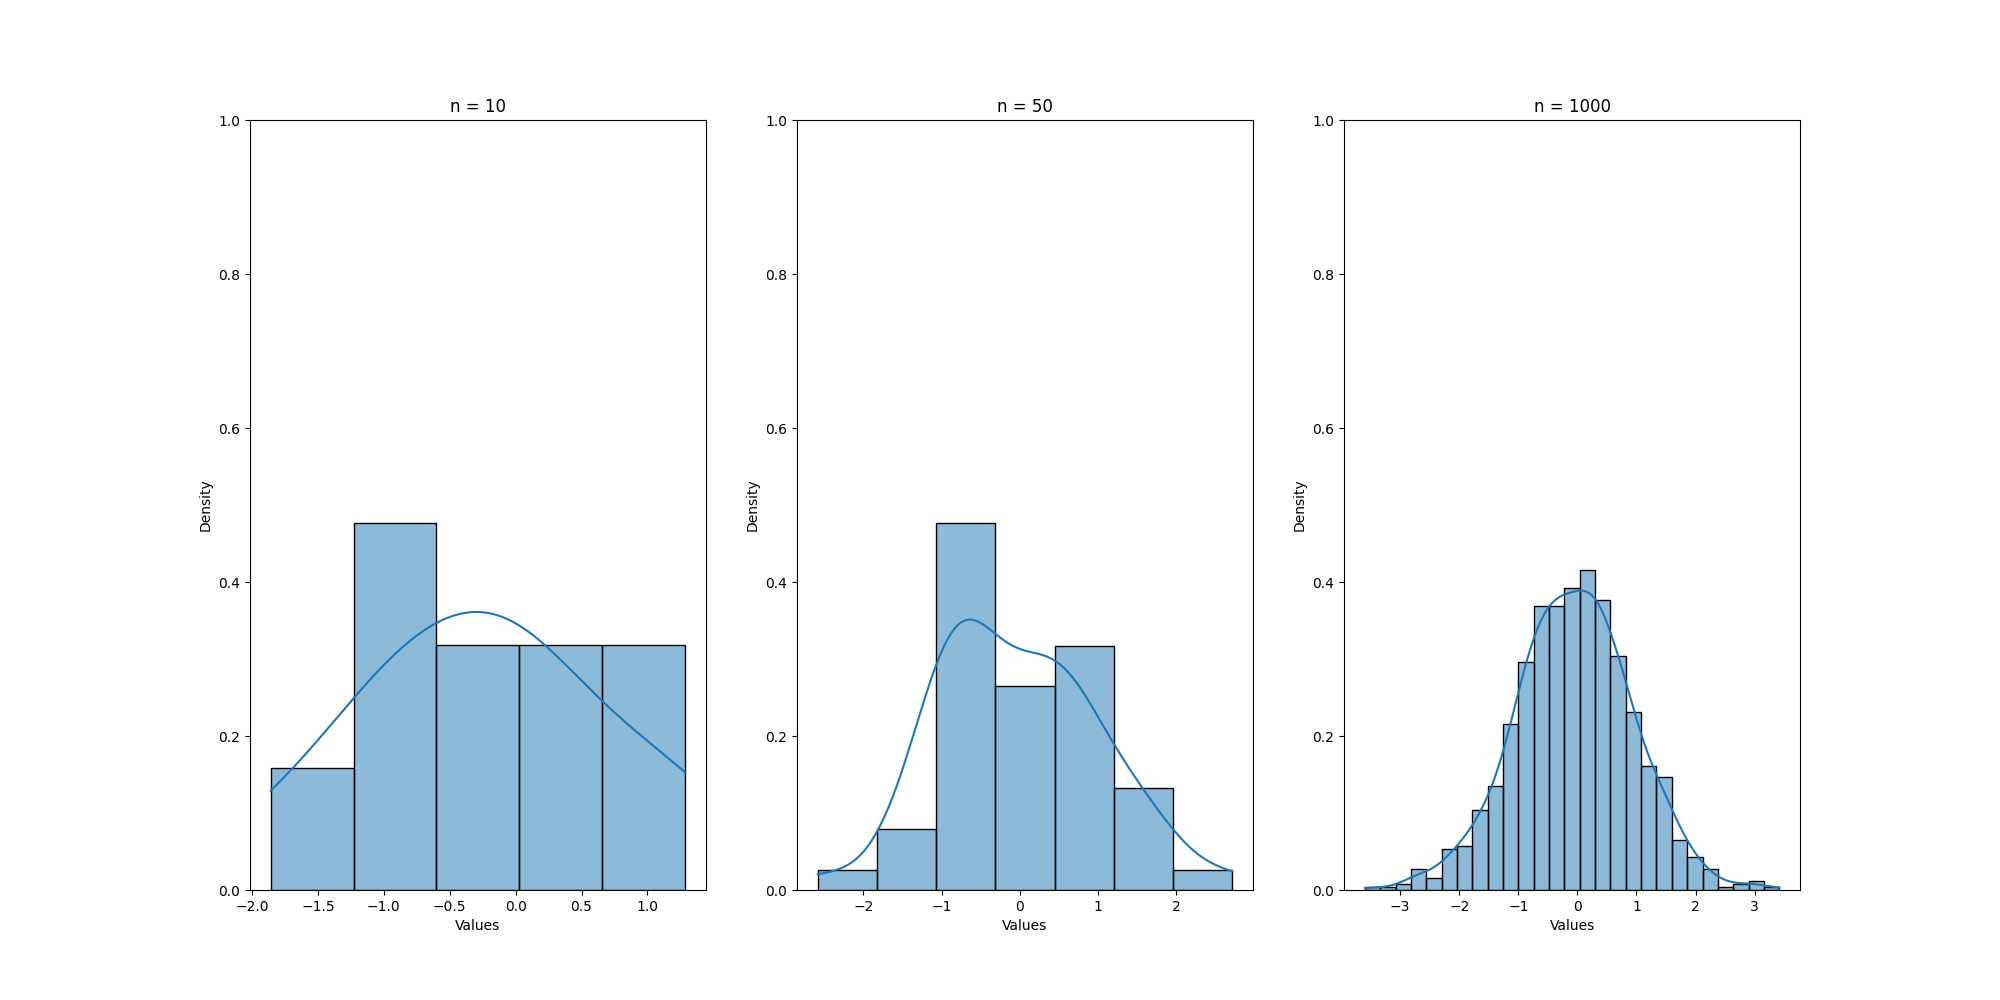
\includegraphics[width = 1.12\linewidth]{graphics/normal.png}
			\caption{Нормальное распределение \ \eqref{eq:normal}}
		\end{center}
	\end{figure}

	\begin{figure}[h!]
		\begin{center}
			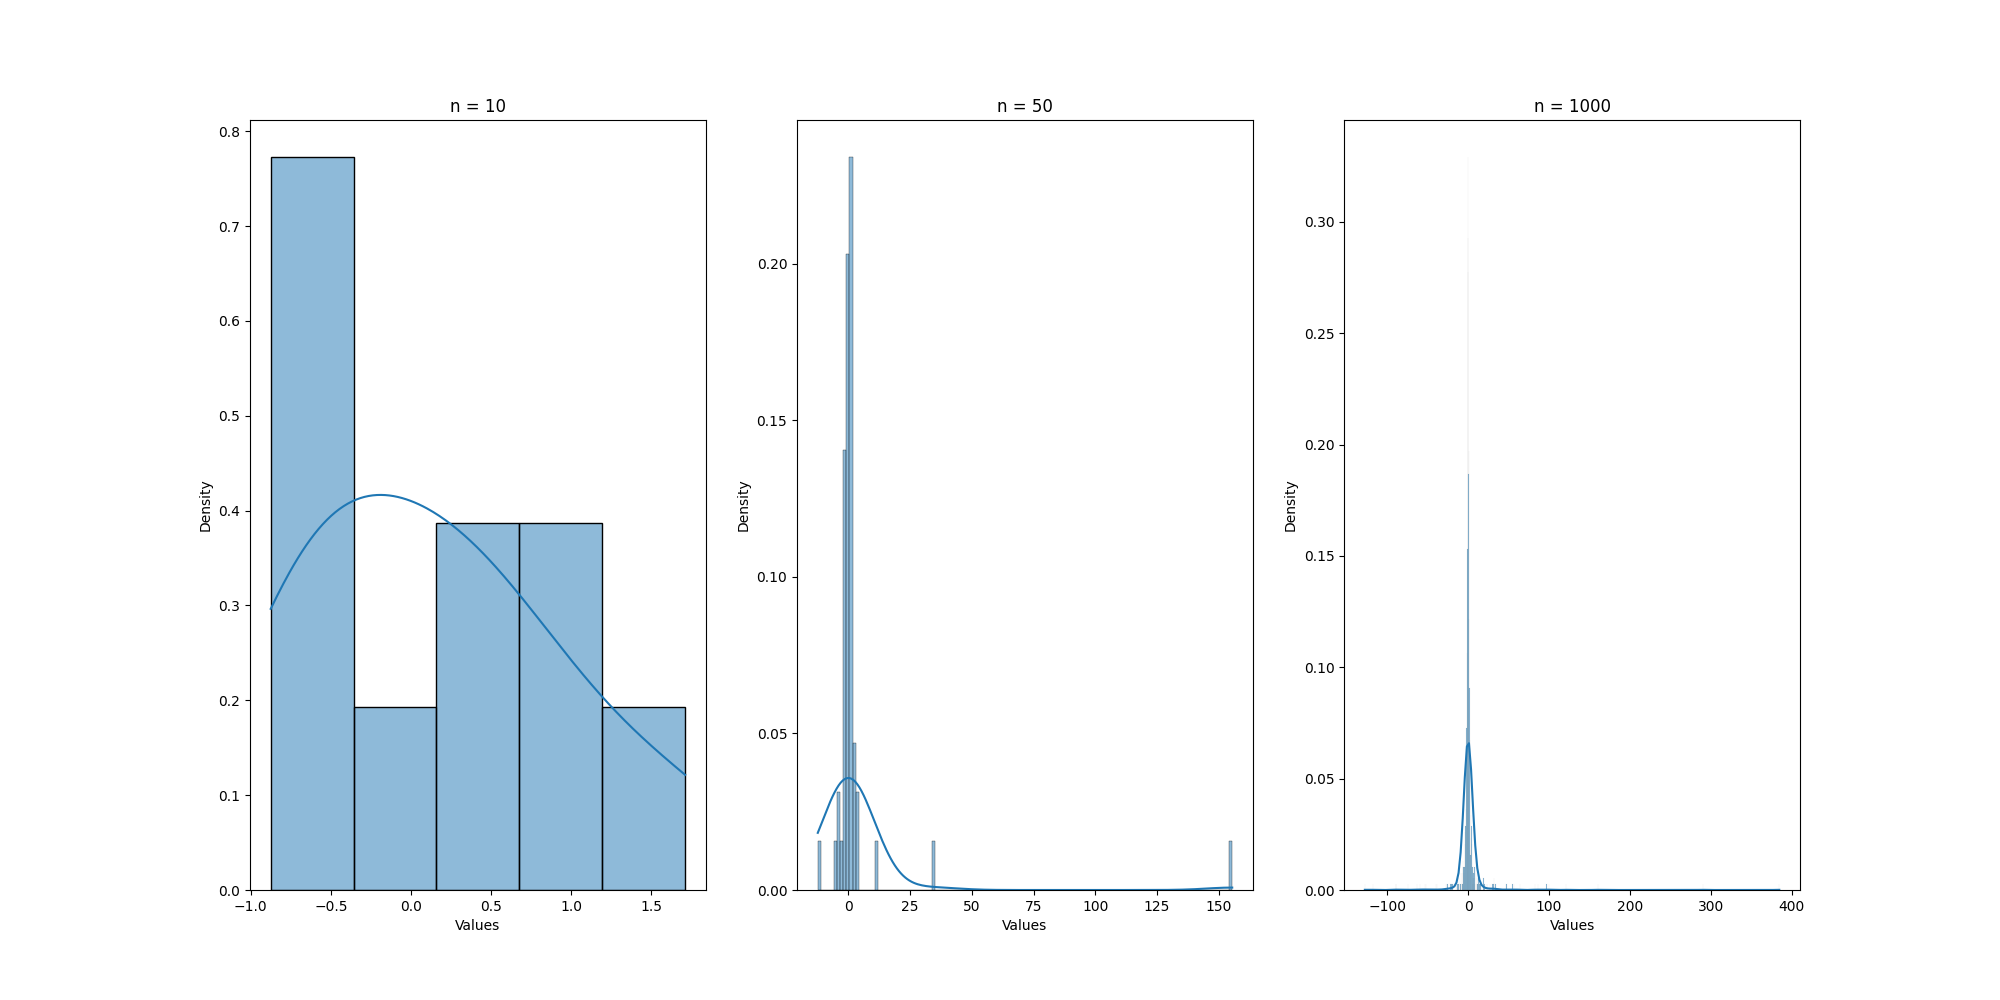
\includegraphics[width = 1.12\linewidth]{graphics/cauchy.png}
			\caption{Распределение Коши \ \eqref{eq:cauchy}}
		\end{center}
	\end{figure}

	\newpage

	\begin{figure}[h!]
		\begin{center}
			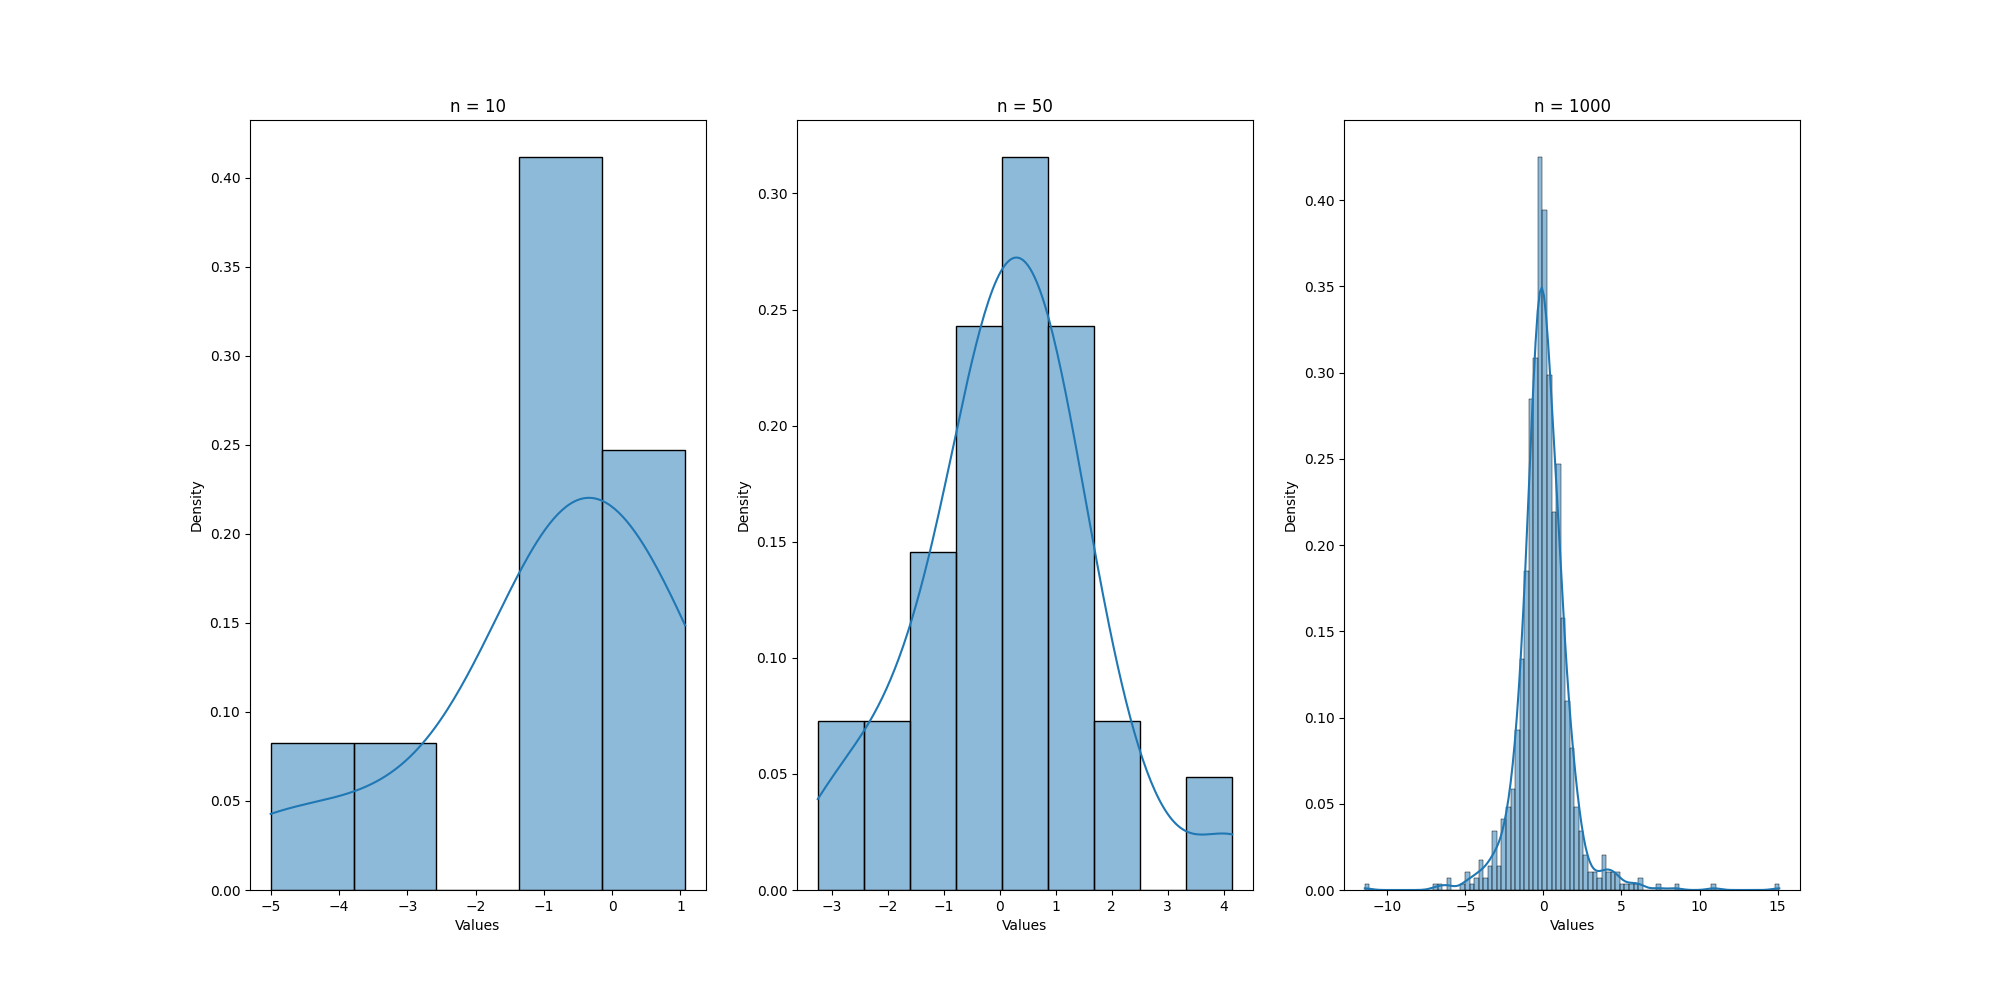
\includegraphics[width = 1.12\linewidth]{graphics/student.png}
			\caption{Распределение Стьюдента \ \eqref{eq:student}}
		\end{center}
	\end{figure}

	\begin{figure}[h!]
		\begin{center}
			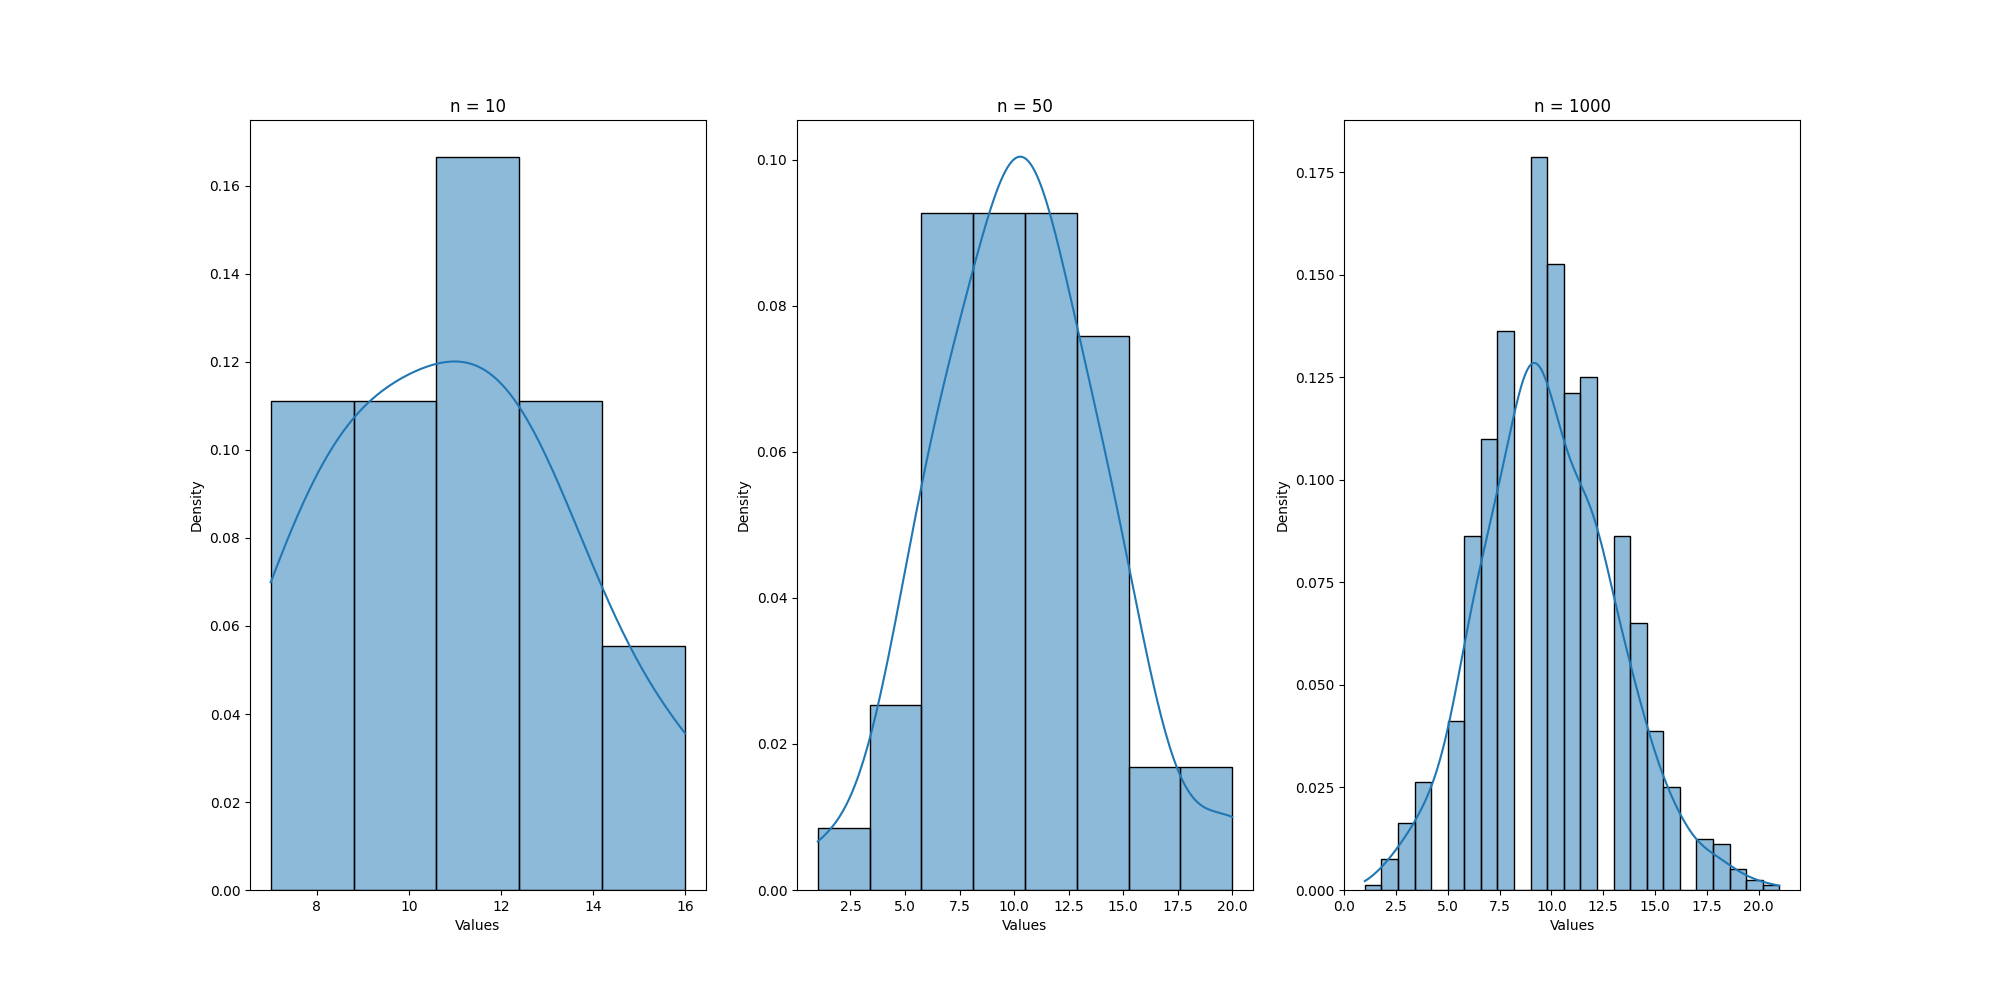
\includegraphics[width = 1.12\linewidth]{graphics/poisson.png}
			\caption{Распределение Пуассона \ \eqref{eq:poisson}}
		\end{center}
	\end{figure}

	\begin{figure}[h!]
		\begin{center}
			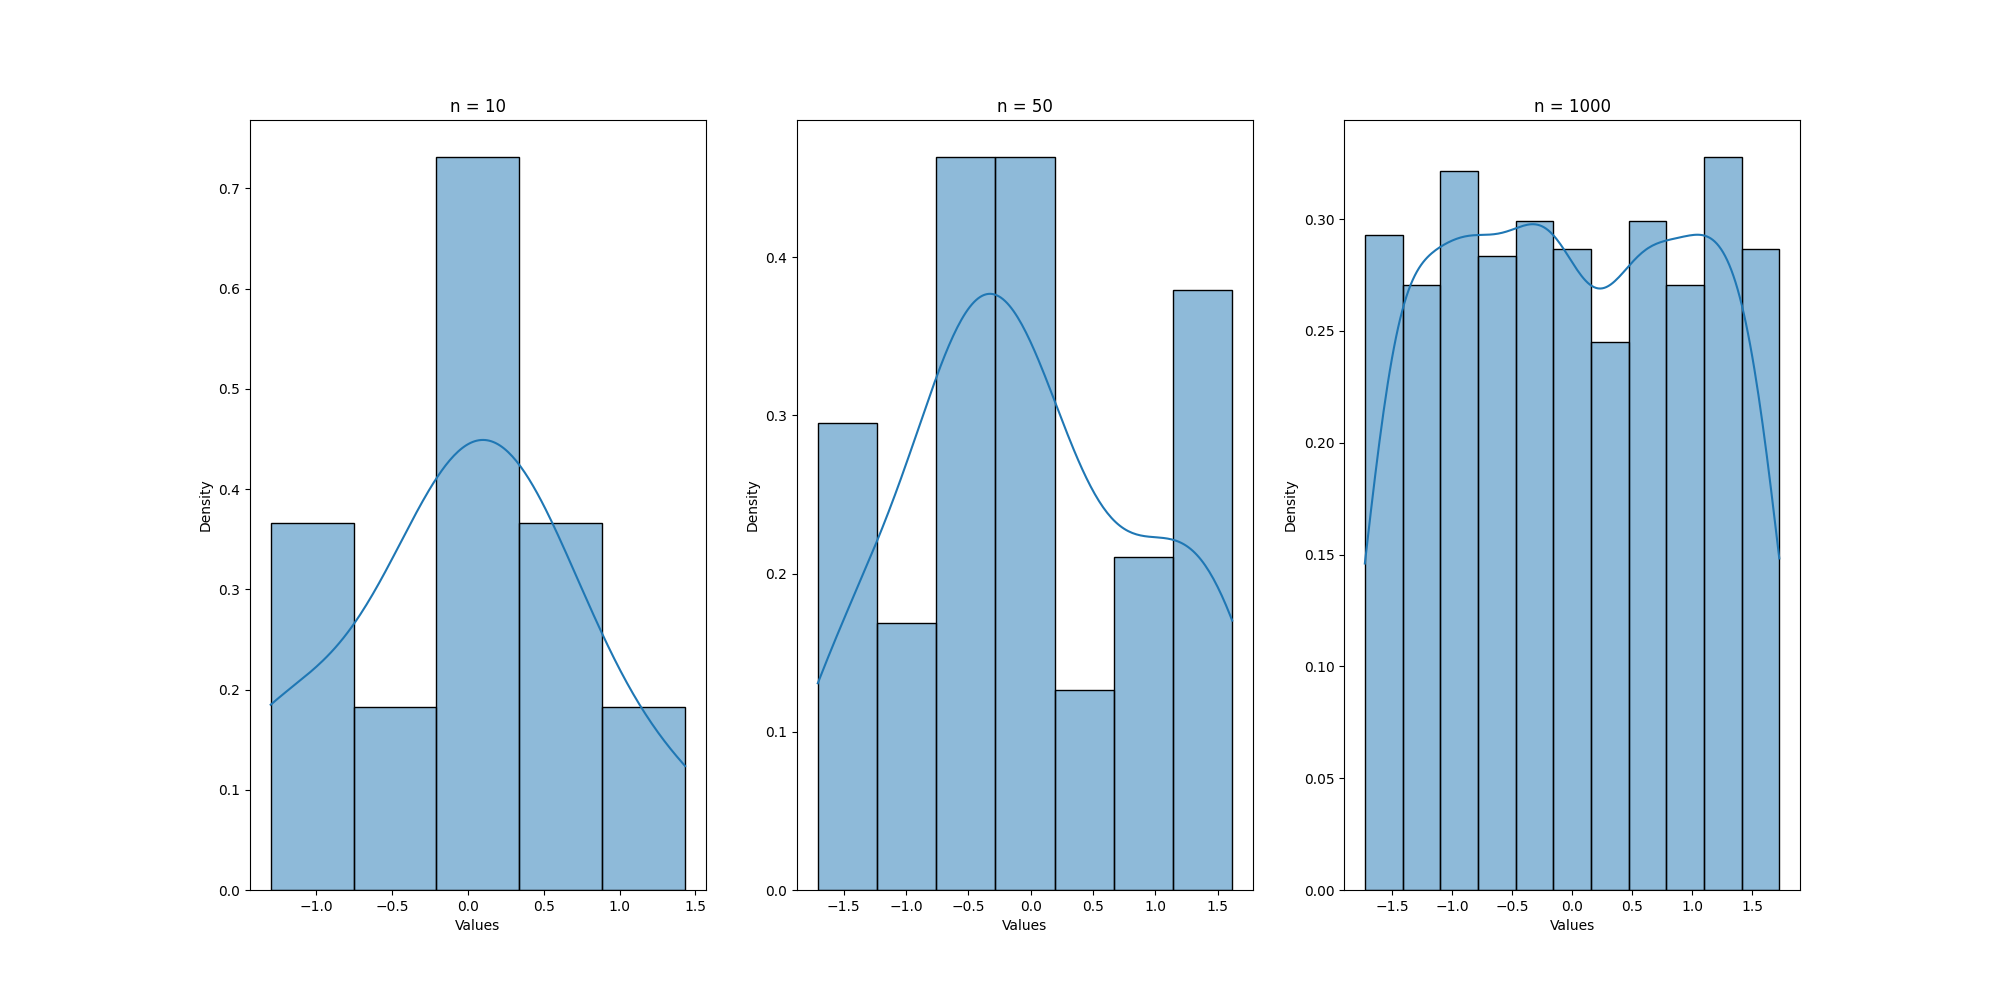
\includegraphics[width = 1.12\linewidth]{graphics/uniform.png}
			\caption{Равномерное распределение \ \eqref{eq:uniform}}
		\end{center}
	\end{figure}

	\newpage

	\subsection{Характеристики положения и рассеяния}

	\begin{table}[h!]
		\centering
		\begin{tabular}{ |c|c|c|c|c|c| }
			\hline
			n = 10 & & & & & \\
			\hline
			&$\overline{x}\ \eqref{eq:mean}$ & $med\ x \ \eqref{eq:median}$ & $z_{R} \ \eqref{eq:half_sum_of_extremal_elements}$ & $z_{Q} \ \eqref{eq:half_sum_of_quartiles}$ & $z_{tr} \ \eqref{eq:trimmed_mean}$\\
			\hline
			$E(z) \ \eqref{eq:expected_value}$ & -0.007982 & -0.004386 & -0.020996 & -0.005516 & -0.006624 \\
			\hline
			$D(z) \ \eqref{eq:dispersion} $ & 0.098372 & 0.143342 & 0.163284 & 0.113910 & 0.163167 \\
			\hline
			n = 50 & & & & & \\
			\hline
			&$\overline{x}\ \eqref{eq:mean}$ & $med\ x \ \eqref{eq:median}$ & $z_{R} \ \eqref{eq:half_sum_of_extremal_elements}$ & $z_{Q} \ \eqref{eq:half_sum_of_quartiles}$ & $z_{tr} \ \eqref{eq:trimmed_mean}$\\
			\hline
			$E(z) \ \eqref{eq:expected_value}$ & 0.003888 & 0.006077 & -0.000529 & 0.002100 & 0.005262 \\
			\hline
			$D(z) \ \eqref{eq:dispersion}$ & 0.010963 & 0.016229 & 0.092033 & 0.013306 & 0.019508 \\
			\hline
			n = 1000 & & & & & \\
			\hline
			&$\overline{x}\ \eqref{eq:mean}$ & $med\ x \ \eqref{eq:median}$ & $z_{R} \ \eqref{eq:half_sum_of_extremal_elements}$ & $z_{Q} \ \eqref{eq:half_sum_of_quartiles}$ & $z_{tr} \ \eqref{eq:trimmed_mean}$\\
			\hline
			$E(z) \ \eqref{eq:expected_value}$ & 0.000841 & 0.001757 & 0.002664 & 0.000549 & 0.001120 \\
			\hline
			$D(z) \ \eqref{eq:dispersion}$ & 0.001003 & 0.001594 & 0.056454 & 0.001218 & 0.002025 \\
			\hline
		\end{tabular}
		\caption{Нормальное распределение}
		\label{table:1}
	\end{table}

	\begin{table}[h!]
		\centering
		\begin{tabular}{ |c|c|c|c|c|c| }
			\hline
			n = 10 & & & & & \\
			\hline
			&$\overline{x}\ \eqref{eq:mean}$ & $med\ x \ \eqref{eq:median}$ & $z_{R} \ \eqref{eq:half_sum_of_extremal_elements}$ & $z_{Q} \ \eqref{eq:half_sum_of_quartiles}$ & $z_{tr} \ \eqref{eq:trimmed_mean}$\\
			\hline
			$E(z) \ \eqref{eq:expected_value}$ & 0.031223 & 0.000157 & 0.091224 & 0.010353 & 0.026922 \\
			\hline
			$D(z) \ \eqref{eq:dispersion} $ & 0.593557 & 0.276924 & 3.039111 & 0.431265 & 1.018721 \\
			\hline
			n = 50 & & & & & \\
			\hline
			&$\overline{x}\ \eqref{eq:mean}$ & $med\ x \ \eqref{eq:median}$ & $z_{R} \ \eqref{eq:half_sum_of_extremal_elements}$ & $z_{Q} \ \eqref{eq:half_sum_of_quartiles}$ & $z_{tr} \ \eqref{eq:trimmed_mean}$\\
			\hline
			$E(z) \ \eqref{eq:expected_value}$ & -0.009060 & -0.001960 & -0.009758 & -0.005885 & -0.001198 \\
			\hline
			$D(z) \ \eqref{eq:dispersion}$ & 0.059867 & 0.024296 & 1.246451 & 0.039833 & 0.119172 \\
			\hline
			n = 1000 & & & & & \\
			\hline
			&$\overline{x}\ \eqref{eq:mean}$ & $med\ x \ \eqref{eq:median}$ & $z_{R} \ \eqref{eq:half_sum_of_extremal_elements}$ & $z_{Q} \ \eqref{eq:half_sum_of_quartiles}$ & $z_{tr} \ \eqref{eq:trimmed_mean}$\\
			\hline
			$E(z) \ \eqref{eq:expected_value}$ & 0.000632 & -0.000889 & 0.005623 & -0.001120 & 0.000454 \\
			\hline
			$D(z) \ \eqref{eq:dispersion}$ & 0.006238 & 0.002337 & 0.038649 & 0.004053 & 0.012341 \\
			\hline
		\end{tabular}
		\caption{Распределение Коши}
		\label{table:2}
	\end{table}

	\begin{table}[h!]
		\centering
		\begin{tabular}{ |c|c|c|c|c|c| }
			\hline
			n = 10 & & & & & \\
			\hline
			&$\overline{x}\ \eqref{eq:mean}$ & $med\ x \ \eqref{eq:median}$ & $z_{R} \ \eqref{eq:half_sum_of_extremal_elements}$ & $z_{Q} \ \eqref{eq:half_sum_of_quartiles}$ & $z_{tr} \ \eqref{eq:trimmed_mean}$\\
			\hline
			$E(z) \ \eqref{eq:expected_value}$ & -0.008120 & 0.003401 & -0.051670 & 0.006376 & -0.006949 \\
			\hline
			$D(z) \ \eqref{eq:dispersion} $ & 0.226164 & 0.168610 & 1.170873 & 0.181303 & 0.391251 \\
			\hline
			n = 50 & & & & & \\
			\hline
			&$\overline{x}\ \eqref{eq:mean}$ & $med\ x \ \eqref{eq:median}$ & $z_{R} \ \eqref{eq:half_sum_of_extremal_elements}$ & $z_{Q} \ \eqref{eq:half_sum_of_quartiles}$ & $z_{tr} \ \eqref{eq:trimmed_mean}$\\
			\hline
			$E(z) \ \eqref{eq:expected_value}$ & 0.001555 & -0.003052 & 0.021573 & -0.002192 & 0.007673 \\
			\hline
			$D(z) \ \eqref{eq:dispersion}$ & 0.023879 & 0.018483 & 1.416933 & 0.018728 & 0.048591 \\
			\hline
			n = 1000 & & & & & \\
			\hline
			&$\overline{x}\ \eqref{eq:mean}$ & $med\ x \ \eqref{eq:median}$ & $z_{R} \ \eqref{eq:half_sum_of_extremal_elements}$ & $z_{Q} \ \eqref{eq:half_sum_of_quartiles}$ & $z_{tr} \ \eqref{eq:trimmed_mean}$\\
			\hline
			$E(z) \ \eqref{eq:expected_value}$ & 0.002647 & 0.000765 & 0.005358 & 0.000688 & 0.000826 \\
			\hline
			$D(z) \ \eqref{eq:dispersion}$ & 0.002287 & 0.001833 & 0.584625 & 0.001828 & 0.004626 \\
			\hline
		\end{tabular}
		\caption{Распределение Стьюдента}
		\label{table:3}
	\end{table}

	\begin{table}[h!]
		\centering
		\begin{tabular}{ |c|c|c|c|c|c| }
			\hline
			n = 10 & & & & & \\
			\hline
			&$\overline{x}\ \eqref{eq:mean}$ & $med\ x \ \eqref{eq:median}$ & $z_{R} \ \eqref{eq:half_sum_of_extremal_elements}$ & $z_{Q} \ \eqref{eq:half_sum_of_quartiles}$ & $z_{tr} \ \eqref{eq:trimmed_mean}$\\
			\hline
			$E(z) \ \eqref{eq:expected_value}$ & 10.060200 & 9.9315 & 10.343 & 9.97575 & 10.0495 \\
			\hline
			$D(z) \ \eqref{eq:dispersion} $ & 1.022076 & 1.364558 & 1.958351 & 1.159037 & 1.690466 \\
			\hline
			n = 50 & & & & & \\
			\hline
			&$\overline{x}\ \eqref{eq:mean}$ & $med\ x \ \eqref{eq:median}$ & $z_{R} \ \eqref{eq:half_sum_of_extremal_elements}$ & $z_{Q} \ \eqref{eq:half_sum_of_quartiles}$ & $z_{tr} \ \eqref{eq:trimmed_mean}$\\
			\hline
			$E(z) \ \eqref{eq:expected_value}$ & 9.997760 & 9.856500 & 10.961500 & 9.904125 & 9.990620 \\
			\hline
			$D(z) \ \eqref{eq:dispersion}$ & 0.101923 & 0.209158 & 0.990268 & 0.147511 & 0.205333 \\
			\hline
			n = 1000 & & & & & \\
			\hline
			&$\overline{x}\ \eqref{eq:mean}$ & $med\ x \ \eqref{eq:median}$ & $z_{R} \ \eqref{eq:half_sum_of_extremal_elements}$ & $z_{Q} \ \eqref{eq:half_sum_of_quartiles}$ & $z_{tr} \ \eqref{eq:trimmed_mean}$\\
			\hline
			$E(z) \ \eqref{eq:expected_value}$ & 10.001017 & 9.998000 & 11.683000 & 9.995250 & 10.006934 \\
			\hline
			$D(z) \ \eqref{eq:dispersion}$ & 0.010374 & 0.001996 & 0.741011 & 0.003759 & 0.020079 \\
			\hline
		\end{tabular}
		\caption{Распределение Пуассона}
		\label{table:4}
	\end{table}

	\begin{table}[h!]
		\centering
		\begin{tabular}{ |c|c|c|c|c|c| }
			\hline
			n = 10 & & & & & \\
			\hline
			&$\overline{x}\ \eqref{eq:mean}$ & $med\ x \ \eqref{eq:median}$ & $z_{R} \ \eqref{eq:half_sum_of_extremal_elements}$ & $z_{Q} \ \eqref{eq:half_sum_of_quartiles}$ & $z_{tr} \ \eqref{eq:trimmed_mean}$\\
			\hline
			$E(z) \ \eqref{eq:expected_value}$ & 0.002619 & 0.013534 & -0.007382 & 0.001860 & 0.003422 \\
			\hline
			$D(z) \ \eqref{eq:dispersion} $ & 0.096635 & 0.220092 & 0.046032 & 0.133492 & 0.163799 \\
			\hline
			n = 50 & & & & & \\
			\hline
			&$\overline{x}\ \eqref{eq:mean}$ & $med\ x \ \eqref{eq:median}$ & $z_{R} \ \eqref{eq:half_sum_of_extremal_elements}$ & $z_{Q} \ \eqref{eq:half_sum_of_quartiles}$ & $z_{tr} \ \eqref{eq:trimmed_mean}$\\
			\hline
			$E(z) \ \eqref{eq:expected_value}$ & 0.001636 & 5.804625-05 & -0.000114 & 0.002965 & 0.004812 \\
			\hline
			$D(z) \ \eqref{eq:dispersion}$ & 0.009758 & 0.029210 & 0.000521 & 0.014602 & 0.018929 \\
			\hline
			n = 1000 & & & & & \\
			\hline
			&$\overline{x}\ \eqref{eq:mean}$ & $med\ x \ \eqref{eq:median}$ & $z_{R} \ \eqref{eq:half_sum_of_extremal_elements}$ & $z_{Q} \ \eqref{eq:half_sum_of_quartiles}$ & $z_{tr} \ \eqref{eq:trimmed_mean}$\\
			\hline
			$E(z) \ \eqref{eq:expected_value}$ & -0.000112 & -0.000167 & -1.956639-05 & 0.000345 & -0.001010 \\
			\hline
			$D(z) \ \eqref{eq:dispersion}$ & 0.000967 & 0.002844 & 5.856189-06 & 0.001470 & 0.001981 \\
			\hline
		\end{tabular}
		\caption{Равномерное распределение}
		\label{table:5}
	\end{table}

	\newpage

	\section{Выводы}
	\vspace{2em}

	В процессе выполнения лабораторной работы был проведен анализ пяти уникальных распределений: нормальное, Коши, Стьюдента, Пуассона и равномерное.
	Были сгенерированы выборки разных объемов для каждого из них - 10, 50 и 1000 элементов.
	Были созданы гистограммы каждого распределения и нанесены на них графики плотности соответствующих распределений, что облегчило наглядное сопоставление формы распределения выборок с их теоретическими аналогами.
	Были также рассчитаны разные показатели положения и рассеяния для каждой выборки, включая выборочную среднюю величину, медиану, полусумму крайних элементов выборки, полусумму квартилей и усеченное среднее.
	Использовалась стандартная формула для оценки дисперсии. \\

	На основании полученных данных были сделаны следующие выводы:

	\begin{enumerate}
		\item В случае нормального распределения, оценки показателей положения и рассеяния становятся ближе к их теоретическим значениям по мере увеличения размера выборки.
		\item Для распределения Коши показатели положения и рассеяния менее стабильны и могут сильно отличаться от теоретических даже при больших размерах выборки.
		\item Распределение Стьюдента при небольших размерах выборки также демонстрирует определенную нестабильность оценок, однако с увеличением размера выборки результаты становятся более точными.
		\item Для распределения Пуассона и равномерного распределения, оценки показателей положения и рассеяния кажутся стабильными при любом объеме выборки. \\
	\end{enumerate}

\end{document}
